\documentclass[12pt,twoside]{article}
\usepackage[dvipsnames]{xcolor}
\usepackage{tikz,graphicx,amsmath,amsfonts,amscd,amssymb,bm,cite,epsfig,epsf,url}
\usepackage[hang,flushmargin]{footmisc}
\usepackage[colorlinks=true,urlcolor=blue,citecolor=blue]{hyperref}
\usepackage{amsthm,multirow,wasysym,appendix}
\usepackage{array,subcaption} 
% \usepackage[small,bf]{caption}
\usepackage{bbm}
\usepackage{pgfplots}
\usetikzlibrary{spy}
\usepgfplotslibrary{external}
\usepgfplotslibrary{fillbetween}
\usetikzlibrary{arrows,automata}
\usepackage{thmtools}
\usepackage{blkarray} 
\usepackage{textcomp}
\usepackage[left=0.8in,right=1.0in,top=1.0in,bottom=1.0in]{geometry}

\input{macros}

\newcommand{\ru}{\rnd{ u}  }
\newcommand{\rd}{\rnd{ d}  }
%\newcommand{\rs}{\rnd{ s}  }
\newcommand{\ri}{\rnd{ i}  }
\newcommand{\re}{\rnd{ e}  }
\newcommand{\rQ}{\rnd{ q}  }
\newcommand{\rC}{\rnd{ c}  }


\begin{document}

\begin{center}
{\large{\textbf{Homework 7}} } \vspace{0.2cm}\\
Due November 12 at 11 pm
\\
\end{center}
\input{hwstatement.tex}\\

\begin{enumerate}

\item (Spider on a wall) There's a spider living on a wall of your living room that has a painting behind which the spider likes to hide. Figure~\ref{fig:wall} shows a diagram of the wall; it is 10 feet high and 10 feet wide.
\begin{figure}[h]
\begin{center}
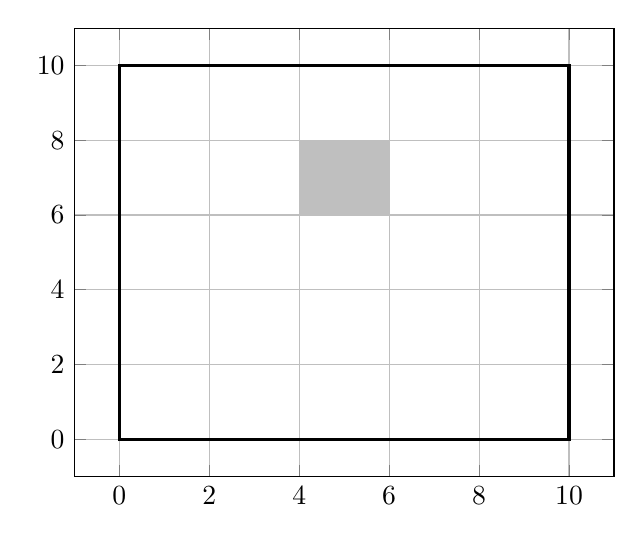
\begin{tikzpicture}
\begin{axis}[grid=major, xtick={0,2,...,10}, ytick={0,2,...,10}, xmin= -1, xmax=11, ymin=-1, ymax=11]
\addplot[ very thick] coordinates
{(0,0) (0,10) (10,10) (10,0) } --cycle;
\addplot[ fill,  lightgray] coordinates
{(4,6) (4,8) (6,8) (6,6) } --cycle;
\end{axis}
\end{tikzpicture}
\end{center}
\caption{Wall and painting (in gray).}
\label{fig:wall}
\end{figure}

After observing the spider for a while you determine that (1) it spends twice the time behind the painting than on the rest of the wall, (2) it never crawls on the painting or leaves the wall, (3) if it is not behind the painting then it is equally likely to be anywhere on the wall. Since you cannot see it behind the painting, you assume that when it is there it is also equally likely to be at any spot.

\begin{enumerate}
\item Model the position of the spider as a bivariate random variable and give its pdf.
\item Compute the pdf of the height at which the spider is located and sketch it.
\item Compute the conditional cdf of the height at which the spider is located, given that you can see it (i.e. it's not under the painting) and sketch it. 
\end{enumerate}

\item (Sonar)
A scientist is trying to determine the depth of the sea at a certain location. She knows that it must be deeper than $5$ km but that is all she knows. To capture this uncertainty she models the depth as uniformly distributed between 5 and 10 km. In order to measure the depth she uses sonar, taking 2 measurements, which we model as two random variables $\rs_1$ and $\rs_2$. If the depth is equal to $x$ then each sonar measurement is uniformly distributed between $x-0.25$ and $x+0.25$. The two measurements are conditionally independent given the depth. 
\begin{enumerate}
%\item Are the two measurements independent? Justify your answer mathematically and explain it intuitively.  
\item Compute and sketch the pdf of the first sonar measurement $\rs_1$. 
\item Compute the conditional pdf of the depth conditioned on the measurements being equal to 7 km and 7.1 km.
\item Compute the joint pdf of the two sonar measurements $\rs_1$ and $\rs_2$. Are the two measurements independent? Justify your answer mathematically and explain it intuitively.
\end{enumerate}

 \item (Exotic fruit) A pomologist is studying a newly-discovered plant that produces edible fruit. They have available 10 specimens, which she measures to obtain the following data:\\
 \\
 {\footnotesize
\begin{tabular}{  |>{\arraybackslash}m{0.25\linewidth} | >{\centering\arraybackslash}m{0.035\linewidth} | >{\centering\arraybackslash}m{0.035\linewidth} |  >{\centering\arraybackslash}m{0.035\linewidth} | >{\centering\arraybackslash}m{0.035\linewidth} | >{\centering\arraybackslash}m{0.035\linewidth} | >{\centering\arraybackslash}m{0.035\linewidth} | >{\centering\arraybackslash}m{0.035\linewidth} | >{\centering\arraybackslash}m{0.035\linewidth} | >{\centering\arraybackslash}m{0.035\linewidth} | >{\centering\arraybackslash}m{0.035\linewidth} | >{\centering\arraybackslash}m{0.035\linewidth} | >{\centering\arraybackslash}m{0.035\linewidth} | }
% \hline
\hline
 %& 1 & 2 & 3 & 4 & 5 & 6 & 7 & 8 & 9 & 10 \\
Fruit weight (kg) & 1.5 & 2.3 & 0.8 & 1.2 & 2.0 & 1.2 & 0.7 & 2.7 & 2.3 & 0.6 \\ 
Stem height (cm) & 20 & 15 & 18 & 19 & 17 & 22 & 21 & 14 & 17 & 22  \\ 
Stem radius (mm) & 8 & 12 &6 & 10 & 17 & 12 & 9 & 14 & 10 & 8  \\ 
Number of leafs & 110 & 94 & 152 & 123 & 78 & 60 & 111 & 83 & 85 & 90  \\ 
Median leaf length (cm) &12 & 21 & 9 & 14 & 19 & 15 & 7 & 29 & 22 & 15  \\ 
\hline
\end{tabular} }
\\

The pomologist wants to use these data to model the conditional pdf of the fruit weight given the other four features. 
\begin{enumerate}
\item Why is it difficult to estimate the conditional pdf using a simple nonparametric estimator where we apply kernel density estimation to a relevant subset of the data?
\item Model all the features as jointly Gaussian and use the model to compute the conditional pdf of the fruit weight for a plant that has a stem height of 15 cm, a stem radius of 20 mm, 120 leafs and median leaf length of 8 cm.
\end{enumerate}

\item (Simulating a random vector) Explain how to simulate a random two-dimensional vector $\rx$ with a joint pdf $f_{\rx}(x)$ that is uniformly distributed in the shaded region. Assume that you have access to independent samples from a uniform distribution in $[0,1]$. Explain your method, justifying why it works. Then implement it and submit the code along with a scatterplot of 1,000 samples.

\begin{figure}[h]
\begin{center}
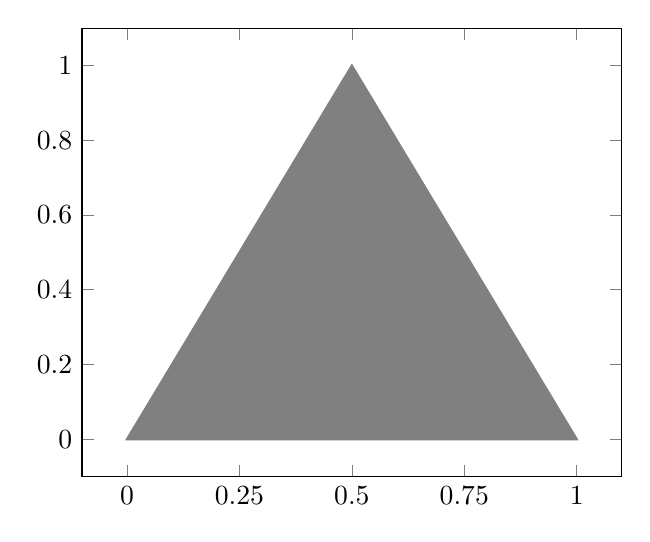
\begin{tikzpicture}
\begin{axis}[xtick={0,0.25,0.5,0.75,1}]%[xlabel=$x$,ylabel=$x$]
\addplot[ thick,fill, gray] coordinates
{ (0.5,1) (1,0) (0,0) } --cycle;
\end{axis}
\end{tikzpicture}
\end{center}
\end{figure}

\end{enumerate}
\end{document}
